\documentclass[a4paper]{article}

\usepackage{a4wide}
\usepackage{amsmath}
\usepackage{amssymb}
\usepackage{amsthm}
\usepackage{enumitem}
    \setlist[enumerate]{label=(\alph*),itemsep=0pt,topsep=0pt}
    \setlist[itemize]{itemsep=0pt,topsep=0pt}
\usepackage{tikz}
\usepackage[utf8]{inputenc}

\theoremstyle{definition}
\newtheorem{problem}{Příklad}
\newtheorem*{ukol}{Domácí úkol}


\begin{document}

\section*{NAIL062 V\&P Logika: 8. cvičení}


\textbf{Témata:}
Struktury a podstruktury. Extenze teorií, extenze o definice. Definovatelné množiny.


\medskip\begin{problem}
    Uvažme $\underline{\mathbb{Z}}_4=\langle\{0,1,2,3\},+,-,0 \rangle$ kde $+$ je binární sčítání modulo $4$ a $-$ je unární funkce, která vrací \emph{inverzní} prvek $+$ vzhledem k \emph{neutrálnímu} prvku $0$.
    \begin{enumerate}        
        \item Je $\underline{\mathbb{Z}}_4$ model teorie grup (tj. je to \emph{grupa})?
        \item Určete všechny podstruktury $\underline{\mathbb{Z}}_4\langle a\rangle$ generované nějakým $a\in \mathbb{Z}_4$.
        \item Obsahuje $\underline{\mathbb{Z}}_4$ ještě nějaké další podstruktury?
        \item Je každá podstruktura $\underline{\mathbb{Z}}_4$ modelem teorie grup?
        \item Je každá podstruktura $\underline{\mathbb{Z}}_4$ elementárně ekvivalentní $\underline{\mathbb{Z}}_4$?
        \item Je každá podstruktura \emph{komutativní} grupy (tj. grupy, která splňuje $x+y=y+x$) také komutativní grupa?
    \end{enumerate}
\end{problem}
 
        
\medskip\begin{problem}
    Buď $\underline{\mathbb{Q}}=\langle\mathbb{Q},+,-,\cdot,0,1 \rangle$ těleso racionálních čísel se standardními operacemi.
    \begin{enumerate}                
        \item Existuje redukt $\underline{\mathbb{Q}}$, který je modelem teorie grup?
        \item Lze redukt $\langle\mathbb{Q},\cdot,1\rangle$ rozšířit na model teorie grup?
        \item Obsahuje $\underline{\mathbb{Q}}$ podstrukturu, která není elementárně ekvivalentní $\underline{\mathbb{Q}}$?
        \item Označmě $Th(\underline{\mathbb{Q}})$ množinu všech sentencí pravdivých v $\underline{\mathbb{Q}}$. Je $Th(\underline{\mathbb{Q}})$ úplná teorie?
    \end{enumerate}
\end{problem}
    

\medskip\begin{problem}
    Mějme teorii $T=\{x=c_1 \vee x=c_2 \vee x=c_3\}$ v jazyce $L=\langle c_1,c_2,c_3\rangle$ s rovností.
    \begin{enumerate}        
        \item Je $T$ (sémanticky) konzistentní?
        \item Jsou všechny modely $T$ elementárně ekvivalentní? Tj. je $T$ kompletní?
        \item Najděte všechny jednoduché úplné extenze $T$.
        \item Je teorie $T'=T\cup\{x=c_1 \vee x=c_4\}$ v jazyce $L=\langle c_1,c_2,c_3,c_4\rangle$ extenzí $T$? Je $T'$ jednoduchá extenze $T$? Je $T'$ konzervativní extenze $T$?
    \end{enumerate}
\end{problem}


\medskip\begin{problem}
Buď $T=\{\neg E(x,x), E(x,y)\to E(y,x), (\exists x)(\exists y)(\exists z)(E(x,y)\wedge E(y,z)\wedge E(x,z)\wedge \neg(x=y\vee y=z\vee x=z)),\varphi\}$ teorie v jazyce $L=\langle E\rangle$ s rovností, kde $E$ je binární relační symbol a $\varphi$ vyjadřuje, že ``existují právě čtyři prvky''.
\begin{enumerate}    
    \item Uvažme rozšíření $L'=\langle E,c\rangle$ jazyka o nový konstantní symbol $c$. Určete počet (až na ekvivalenci) teorií $T'$ v jazyce $L'$, které jsou extenzemi teorie $T$. 
    \item Má $T$ nějakou \emph{konzervativní} extenzi v jazyce $L'$? Zdůvodněte.
\end{enumerate}
\end{problem}


\medskip\begin{problem}
Nechť $T=\{x=f(f(x)),\varphi, c_1 \ne c_2\}$ je teorie jazyka $L=\langle f,c_1,c_2\rangle$ s rovností, kde $f$ je unární funkční, $c_1,c_2$ jsou konstantní symboly a axiom $\varphi$ vyjadřuje, že ``existují právě $3$ prvky''.
\begin{enumerate}    
    \item Určete, kolik má teorie $T$ navzájem neekvivalentních jednoduchých kompletních extenzí. Napište dvě z nich. {\it (3b)}
    \item Nechť $T'=\{x=f(f(x)),\varphi,f(c_1)\ne f(c_2)\}$ je teorie stejného jazyka, axiom $\varphi$ je stejný jako výše. Je $T'$ extenze $T$? Je $T$ extenze $T'$? Pokud ano, jde o konzervativní extenzi? Uveďte zdůvodnění. {\it (2b)}
\end{enumerate}
\end{problem}



\medskip\begin{problem}
Nechť $T_n = \{c_i \neq c_j | 1 \leq i < j \leq n\}$ označuje teorii jazyka $L_n = \langle c_1, \dots, c_n \rangle$ s rovností, kde $c_1, \dots, c_n$ jsou konstantní symboly.
\begin{enumerate}    
    \item Pro dané konečné $n \geq 1$ určete počet modelů konečné velikosti $k$ teorie $T_n$ až na izomorfismus. Určete počet spočetných modelů teorie $T_n$. 
    \item Pro jaké dvojice hodnot $n$ a $m$ je $T_n$ extenzí $T_m$? Pro jaké je konzervativní extenzí? Zdůvodněte.
\end{enumerate}
\end{problem}


\medskip\begin{problem}
Buď $T'$ extenze teorie $T=\{(\exists y)(x+y=0),(x+y=0)\wedge (x+z=0)\rightarrow y=z\}$ v jazyce $L=\langle +,0,\le\rangle$ s rovností o definice $<$ a unárního $-$ s axiomy
\begin{align*}
    -x=y\ \ &\leftrightarrow\ \ x+y=0\\
    x<y\ \ &\leftrightarrow\ \ x\le y\ \wedge\ \neg(x=y)
\end{align*}
Najděte formule v jazyce $L$, které jsou ekvivalentní v $T'$ s následujícími formulemi.
\begin{enumerate}    
    \item $x+(-x)=0$
    \item $x+(-y)<x$
    \item $-(x+y)<-x$
\end{enumerate}
\end{problem}


\medskip\begin{problem}
Mějme jazyk $L=\langle F \rangle$ s rovností, kde $F$ je binární funkční symbol. Najděte formule definující následující množiny (bez parametrů):
\begin{enumerate}
    \item interval $(0,\infty)$ v $\mathcal A=\langle\mathbb R, \cdot\rangle$ kde $\cdot$ je násobení reálných čísel,
    \item množina $\{(x, 1/x)\mid x\neq 0\}$ ve stejné struktuře $\mathcal A$,
    \item množina všech nejvýše jednoprvkových podmnožin $\mathbb N$ v $\mathcal B=\langle\mathcal P(\mathbb N),\cup\rangle$,
    \item množina všech prvočísel v $\mathcal C=\langle \mathbb N\cup\{0\}, \cdot\rangle$.
\end{enumerate}
\end{problem}


\medskip\begin{problem} % move to tutorial 13?
Nechť $\mathcal{A}=\langle\mathbb{Z},\mathrm{abs}^A \rangle$ je struktura jazyka $L=\langle \mathrm{abs} \rangle$ s rovností, kde $\mathrm{abs}$ je unární funkční symbol a $\mathrm{abs}^A$ je funkce absolutní hodnoty v $\mathbb{Z}$.
\begin{enumerate}
    \item Nalezněte příklady $(i)$ netriviální (t.j. jiné než $\emptyset$ a $\mathbb{Z}$) množiny definovatelné v $\mathcal{A}$ bez parametrů a $(ii)$ množiny nedefinovatelné v $\mathcal{A}$ bez parametrů.
    \item Mějme $L$-strukturu $\mathcal{B}=\langle\mathbb{N},\mathrm{id} \rangle$, kde $\mathrm{id}$ je identita. Je $Th(\mathcal{A})$ extenzí $Th(\mathcal{B})$?
\end{enumerate}
\end{problem}


\medskip\begin{ukol}[2 body]
    Nechť $T$ je teorie jazyka $L=\langle T \rangle$ s rovností, kde $T$ je ternární relační symbol, s axiomy:
    \begin{align*}
        T(x,y,z)&\to x\ne y \wedge y\ne z \wedge x\ne z \\
        T(x,y,z)&\to T(y,x,z)\wedge T(y,z,x)\wedge T(z,y,x)\wedge T(z,x,y)\wedge T(x,z,y)\\
        x\ne y &\to (\exists z)(T(x,y,z)\wedge(\forall u)(T(x,y,u)\to u=z))
    \end{align*}
    Modely teorie $T$ jsou tzv. \emph{Steinerovy systémy trojic}, v našem případě uspořádaných. Uvažme model $\mathcal{F}=\langle \{1,2,\dots,7\},T^F\rangle$ teorie $T$ na obrázku (tzv. \emph{Fanova rovina}), kde každá ``přímka'' reprezentuje trojici prvků, jež jsou v relaci $T^F$ v libovolném pořadí, tedy $T^F=\{(2,4,6),(6,2,4),\dots\}$.
    \begin{center}
        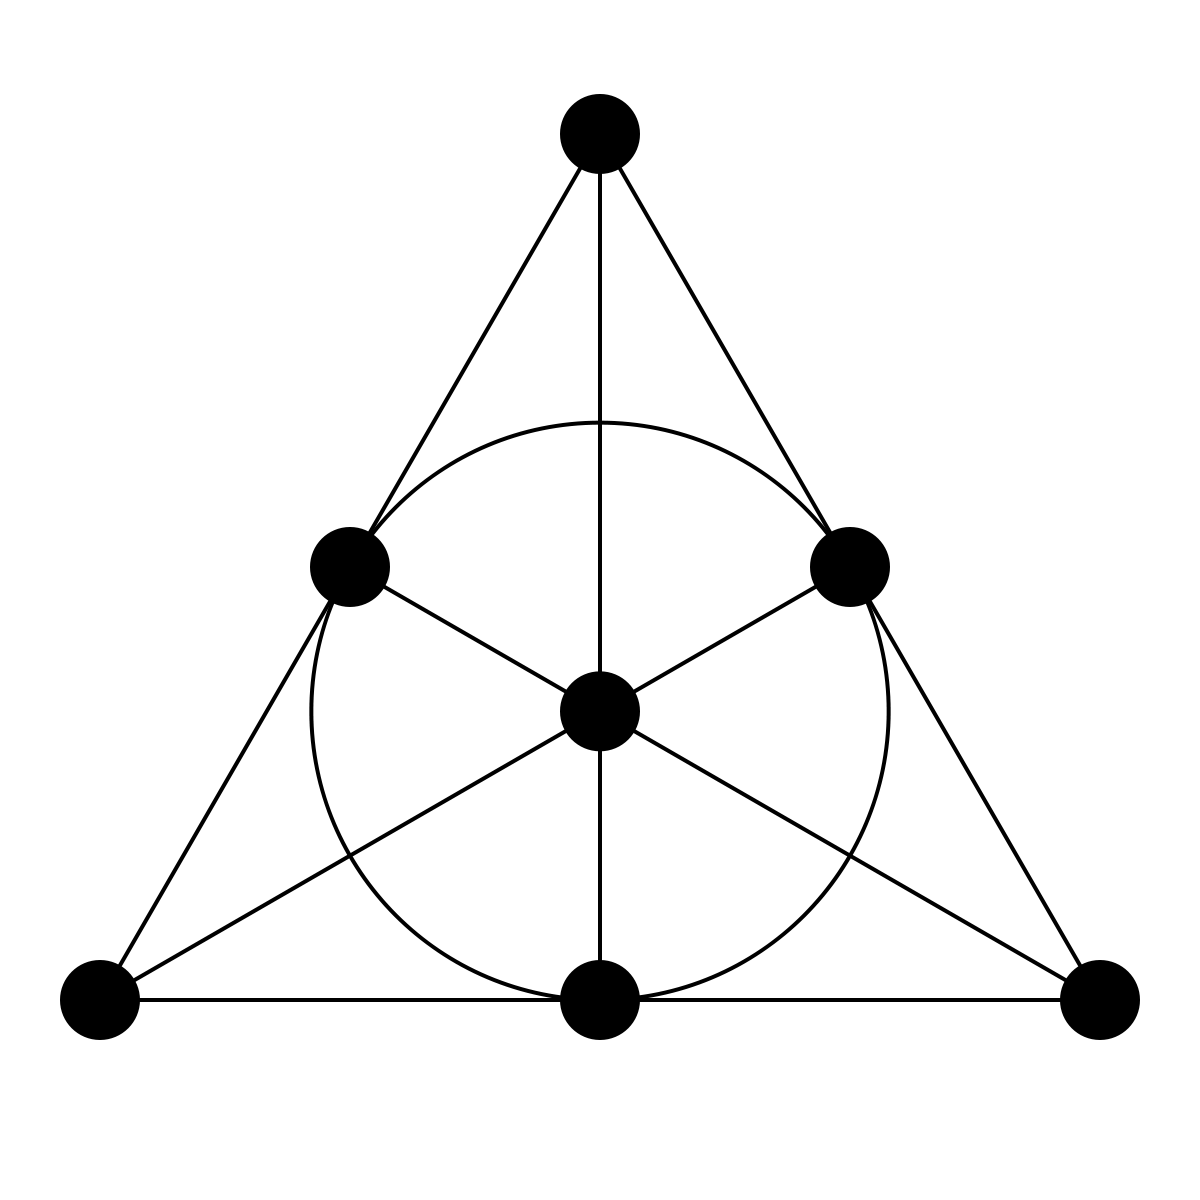
\includegraphics[height=4cm]{files/fano.png}  
    \end{center}
    \begin{enumerate}        
        \item Nalezněte co nejmenší množinu parametrů $A$, která v modelu $\mathcal{F}$ umožňuje definovat libovolný jeho prvek (formulí jazyka $L$). Pro každý prvek napište příslušnou definující formuli (s dosazenými parametry). Zdůvodněte, proč je $A$ nejmenší možná.
        \item Jsou teorie $T'=T \cup \{f(x,y)=z \leftrightarrow T(x,y,z)\}$ a $T''=T\cup \{f(x,y)=z \leftrightarrow T(x,y,z) \vee (x=y \wedge y=z)\}$, kde $f$ je nový binární funkční symbol, (korektními) extenzemi teorie $T$ o definici? Uveďte zdůvodnění.
    \end{enumerate} 
\end{ukol}


\end{document}